\subsection{Generating components}
% Introduce the different components, and describe that each component has different parameters that are described in each section
The proposed system consists of three different components. The first is the terrain. This terrain forms the basis of the landscape on which different features can be placed. The second component consists of water features. These water features, which consist of rivers and ponds, are generated based on a number of control points which are placed onto the terrain. Thirdly, the last component of the system is the placement of vegetation. Vegetation consists of different type of plants, ranging from small bushes to large trees. The generation of each component can be described with a number of parameters. While some parameters would be dependent on the initial settings of the terrain, others can wildly influence the type of landscape created.

In this subsection, the generation of the different components is described in isolation from each other, as well as the parameters required for each component. For each parameter, a description is given what the parameter does in the generation of the component, and how the system can interact with the parameter.

\subsubsection{Terrain}
% Describe what algorithm is chosen and why
In our design, we have chosen to generate terrain using Fractal noise using Perlin noise \cite{musgrave_synthesis_1989}. The advantage of using noise functions is that the calculation of each separate point can be performed in parallel. Each chunk can be generated independent of other chunks.
% Describe the alternative Diamond Square method, and why it does not work correctly with the chunk system
The main downside of using the previously mentioned midpoint displacement algorithm in our architecture is in the chunk system. When generating a chunk with midpoint displacement, the vertices depend on their neighbours and a random offset. In different chunks, these offsets do not correspond to the same values, resulting in different height values for vertices along the edges of neighbouring chunks. To solve this, the height values of vertices can be calculated using the different chunks, but this creates a dependency between chunks.

% Show how the terrain is generated
The terrain is generated on a 2D grid of vertices. For each octave, a separate random 2D offset is generated to be used in the Perlin noise function. This offset is scaled and translated by the scale and position of the vertex in the grid. These coordinates are evaluated using Perlin noise and scaled by the amplitude. The sum of these values is the resulting value in the height map.
To properly overlap different chunks, the last value of each heightmap is scaled to use the same coordinates as the first value of the neighbouring chunk.

% Describe the parameters of the system, and how they are used to create the heightmap.
The parameters that influence the algorithm are shown in table \ref{tab:perlin-parameters}. In this table we make a distinction between parameters that are set by the system because they are constant or implicit based on other systems such as the chunk system, and parameters that can be influenced by a designer.
The width and depth of the system will be fixed, since the amount of vertices in a chunk is deemed to be constant. The offset and seed are implicit in the execution of the program, since the offset is defined by which chunk will be generated and the seed is constant per generation of the system, to provide the same base noise offsets for all chunks.

\begin{table}[ht]
\begin{tabularx}{\linewidth}{|l|l|l|X|}
\hline
Name & Type & Bounds & Description\\
\hline
Width & Int & $\geq 1$ & The width of the heightmap in vertices\\

Height & Int & $\geq 1$ & The depth of the heightmap in vertices\\

Offset & Vec2Int & $\mathbb{Z}^2$ & The chunk coordinates of the generating chunk\\

Seed & Int & $\mathbb{Z}$ & The seed that initialises the random number generator\\

\hline

Scale & Float & $> 0$ & The initial frequency of the noise on the terrain\\

Octaves & Int & $\geq 1$ & How many iterations of the fractal function is applied\\

Persistance & Float & $\geq 0$ & How much the amplitude of the noise is reduced multiplicatively each octave \\

Lacunarity & Float & $\geq 0$ & How much the frequency of the noise is increased multiplicatively each octave \\
\hline

\end{tabularx}
\caption{The parameters used in the fractal noise algorithm. The top section contains constant or implicit parameters, the lower part contains parameters used by the designer.}
\label{tab:perlin-parameters}
\end{table}

% Parameter analysis

% Texturing (Still to be implemented)

\subsubsection{Rivers and ponds}
% The generation of rivers and ponds consist of 2 separate tasks.
The generation of rivers and ponds consist of 2 separate tasks. The first step is to plan the route or shape of the river. After that, the path can be combined with a profile to generate the water.
% First the path of the river needs to be established. This is done by placing points.
% These points form a curve that is used to, together with a curve profile, generate a fat mesh that can be added to the curve.
When the path of the river has been defined, a bezier curve is plotted through the points. When a pond is generated, the end of the curve is connected to the start. Like the system proposed by Huijser\cite{huijser_procedural_2010}, the curve is transformed into a mesh, the fat curve, that can be used in other stages of the program. To transform the path of a river to a fat curve, each curve point is given a width with which a line is constructed perpendicular to the curve. The line creates a triangle mesh with triangles between the curve points. When generating a pond, the middle of the curve is established by taking the average position of all points. The triangles of the mesh are defined by the middle of the curve and two subsequent curve points. Using this fat curve we can check whether a point is inside or outside the curve, and by calculating the barycentric coordinates of a point, the location of that point in the cross-section of the curve is derived. This coordinate can be used with the profile to derive the depth of the river at that location.

% Parameters of path planning

% Parameters of fat curve creation
The parameters that describe the creation of the fat curve are shown in Table \ref{tab:river-fatcurve-parameters}

% Parameter table fatcurve
\begin{table}[ht]
\begin{tabularx}{\linewidth}{|l|l|l|X|}
\hline
Name & Type & Bounds & Description\\
\hline

tangentLength & float & $\mathbb{R}$ & How far the tangents of the bezier curve are scaled. \\

CurvePoint.Direction & Vec3 & $\mathbb{R}^3$ & For each point, the gradient along the curve\\

MeshSubdivisions & int & $\geq 0$ & How many points are interpolated between curvePoints\\

\hline

CurvePoint.Position & Vec3 & $\mathbb{R}^3$ & For each point in the curve, the position in the world\\

CurvePoint.width & float & $> 0$ & For each point, the width of the river along the point\\

closed & boolean & T/F & Whether the curve describes a river (F) or a pond (T) \\
\hline

\end{tabularx}
\caption{The parameters used for generating a fat curve}
\label{tab:river-fatcurve-parameters}
\end{table}

\subsubsection{Placing vegetation}
% Placing vegetation has to adhere to a few rules
In the system, we introduce two different types of placing vegetation. The first method uses the Poisson Disk Distribution to generate points that have a minimum distance from each other. To generate the points, the paper of Bridson \cite{bridson_fast_2007} is used. We have expanded this initial algorithm so that it is able to be used with multiple types of points, where each type of point has a different minimal distance. This approach can be used to generate multiple different types of vegetation.

To generate different types of vegetation, we separate the types of vegetation into different layers, similar to the solution provided by do Nascimento et al. \cite{do_nascimento_gpu-based_2018}. For each separate layer, points are randomly generated. Based on the paper of Bridson, we use a 2-dimensional grid to store the points, with the size of each grid cell being equal to $d / \sqrt{2}$, where $d$ is the minimum distance of two points, which is twice the radius of the object on the layer. Given a boundary where the points lie, the algorithm places points around already generated points until there is no point that can be the neighbour of a new point.

The parameters that describe the placement of points on a single layer are shown in table \ref{tab:pdd-single-layer}. The retries parameter is constant, and a value of 30 is typically used.\\

% Parameter table single-layer PDD
\begin{table}[ht]
\begin{tabularx}{\linewidth}{|l|l|l|X|}
\hline
Name & Type & Bounds & Description\\
\hline

bounds & AABB & Area > 0 & The area wherein objects can be placed. \\
\hline

radius & float & $> 0$ & The radius of an object, or half the minimum distance between points. \\

\hline

retries & int & $\geq 0$ & How many times an already generated point tries to generate an adjacent point until it fails. \\
\hline

\end{tabularx}
\caption{The parameters used for generating a PDD layer}
\label{tab:pdd-single-layer}
\end{table}

To combine multiple layers generated by the PDD, we generate all layers from large to small, and when each layer is generated, all points are filtered by checking if there is overlap with a larger layer. In our system, we can assign a different radius for objects in the same layer as objects in a lower layer. The justification for this is as follows: When placing trees in an environment, their canopies cannot overlap but smaller objects, such as bushes, can be placed within the radius of the canopy but are still blocked by the size of the trunk.

As different layers have different radii, their 2-dimensional grid structure have different sizes. While in the single layer algorithm we only had to check the 8 neighbours of a cell, the size of the neighbourhood differs when different sized grids are used. The radius of the neighbourhood equals $\lceil (r_1 + r_2) / cell\_size_1 \rceil$, with $r_1, cell\_size_1$ corresponding to the larger layer and $r_2$ being the radius of the smaller layer.

The parameters used in the Multi-layer PDD algorithm are shown in table \ref{tab:pdd-multi-layer}. For each layer of the input, the algorithm returns the positions that do not overlap with higher layers.

% Parameter table Multi-layer PDD
\begin{table}[ht]
\begin{tabularx}{\linewidth}{|l|l|l|X|}
\hline
Name & Type & Bounds & Description\\
\hline

bounds & AABB & Area $> 0$ & The area wherein objects can be placed.\\
\hline

layers & Layer[] & size $> 0$ & The different layers of object used in the algorithm.\\
\hline

Layer.layerRadius & float & $> 0$ & The radius of the object within the same layer.\\
\hline

Layer.innerRadius & float & $> 0$ & The radius of the object when checking lower layers.\\
\hline

retries & int & $\geq 0$ & How many times an already generated point tries to generate an adjacent point until it fails. \\
\hline

\end{tabularx}
\caption{The parameters used for generating multiple PDD layers}
\label{tab:pdd-multi-layer}
\end{table}

Our second approach follows the method proposed by Lane et al. \cite{lane_generating_2002}, which uses a probability density function to randomly place objects. Each object placed modifies the probability function with a kernel which has a circular influence on the probability function. The kernel is defined by a radius and a curve, where the value of the curve is equal to the ratio that the probability function will change. Examples of kernels are shown in Figure \ref{fig:deformation_kernel_example}. When using kernel C from this example, new objects have a lower probability to be placed near other objects. Alternatively, using kernel A increases the probability of a new object being placed close to another object.

\begin{figure}
    \centering
    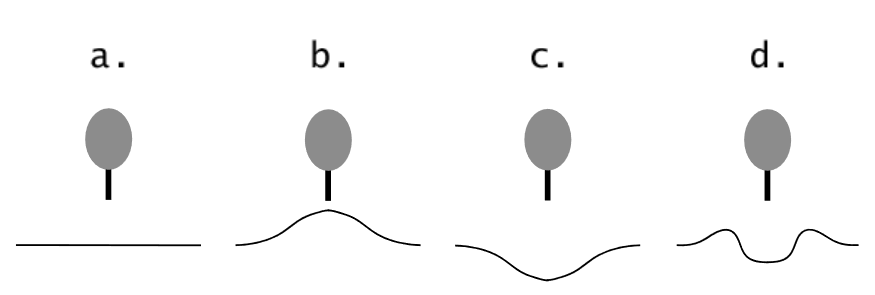
\includegraphics[width=0.9\linewidth]{figures/deformation_kernel_example.png}
    \caption{Examples of kernels that can be used in the deformation kernel algorithm, from \cite{lane_generating_2002}.}
    \label{fig:deformation_kernel_example}
\end{figure}

\todo{Fix formatting of table}
% Parameter table Deformation kernel
\begin{table}[ht]
\begin{tabularx}{\linewidth}{|l|l|l|X|}
\hline
Name & Type & Bounds & Description\\
\hline

bounds & AABB & Area $> 0$ & The area wherein objects can be placed.\\
\hline

deformationObject & DeformationKernel & & The deformation kernel used in updating the density function.\\
\hline

DeformationKernel.curve & AnimationCurve & $f(x) \in [0, 1]$ & The function that is used to deform the probability density function.\\
\hline

DeformationKernel.radius & float & $> 0$ & The size of the influence of the deformation kernel.\\
\hline

iterations & int & $\geq 0$ & The amount of objects to be placed.\\
\hline

fieldSize & int & $> 0$ & The size of the array used as probability density function.\\
\hline

\end{tabularx}
\caption{The parameters used for placing objects with a deformation kernel}
\label{tab:deformation-kernel}
\end{table}

\todo{Table for deformation kernel parameters}

% Elaborate PDD and explain second algorithm

% - Vegetation can be separated into a few different layers, representing different kinds of plants (trees, bushes and grass)\

% - Each piece of vegetation has to be placed a minimum distance apart from each other plant.

% - Vegetation from different layers should not overlap

% - The distance of a plant on layer X is not necessarily equal to the distance of layer Y (e.g. canopy of trees exists on tree layer, but on lower layers the trunk of the tree applies.

% Multilevel PDD placement

% Deformation kernel
